% !TEX root = ./docs.tex

Bei der Implementierung wird Java 11 eingesetzt.
\subsection{Server}
Einstiegspunkt des Servers ist der Serverbootstrapper. Dieser erstellt einen neuen Thread mit einem neuen Server. 
\lstinputlisting[linerange={7-11}, firstnumber=7]{../src/main/java/vs/chat/server/ServerBootstrapper.java}
Der Server erstellt die Listener, die die zu empfangenen Pakete behandeln werden. Anschließend werden die Filter erstellt, die bestimmen, ob ein Paket gehandelt oder ignoriert werden soll (z.B. bei rekursiven Broadcasts).
\lstinputlisting[linerange={64-80}, firstnumber=64]{../src/main/java/vs/chat/server/Server.java}

Die Listener und die Filter werden in einen ServerContext gepackt, der allen Threads geteilt wird.

\begin{figure}[h]
    \centering
    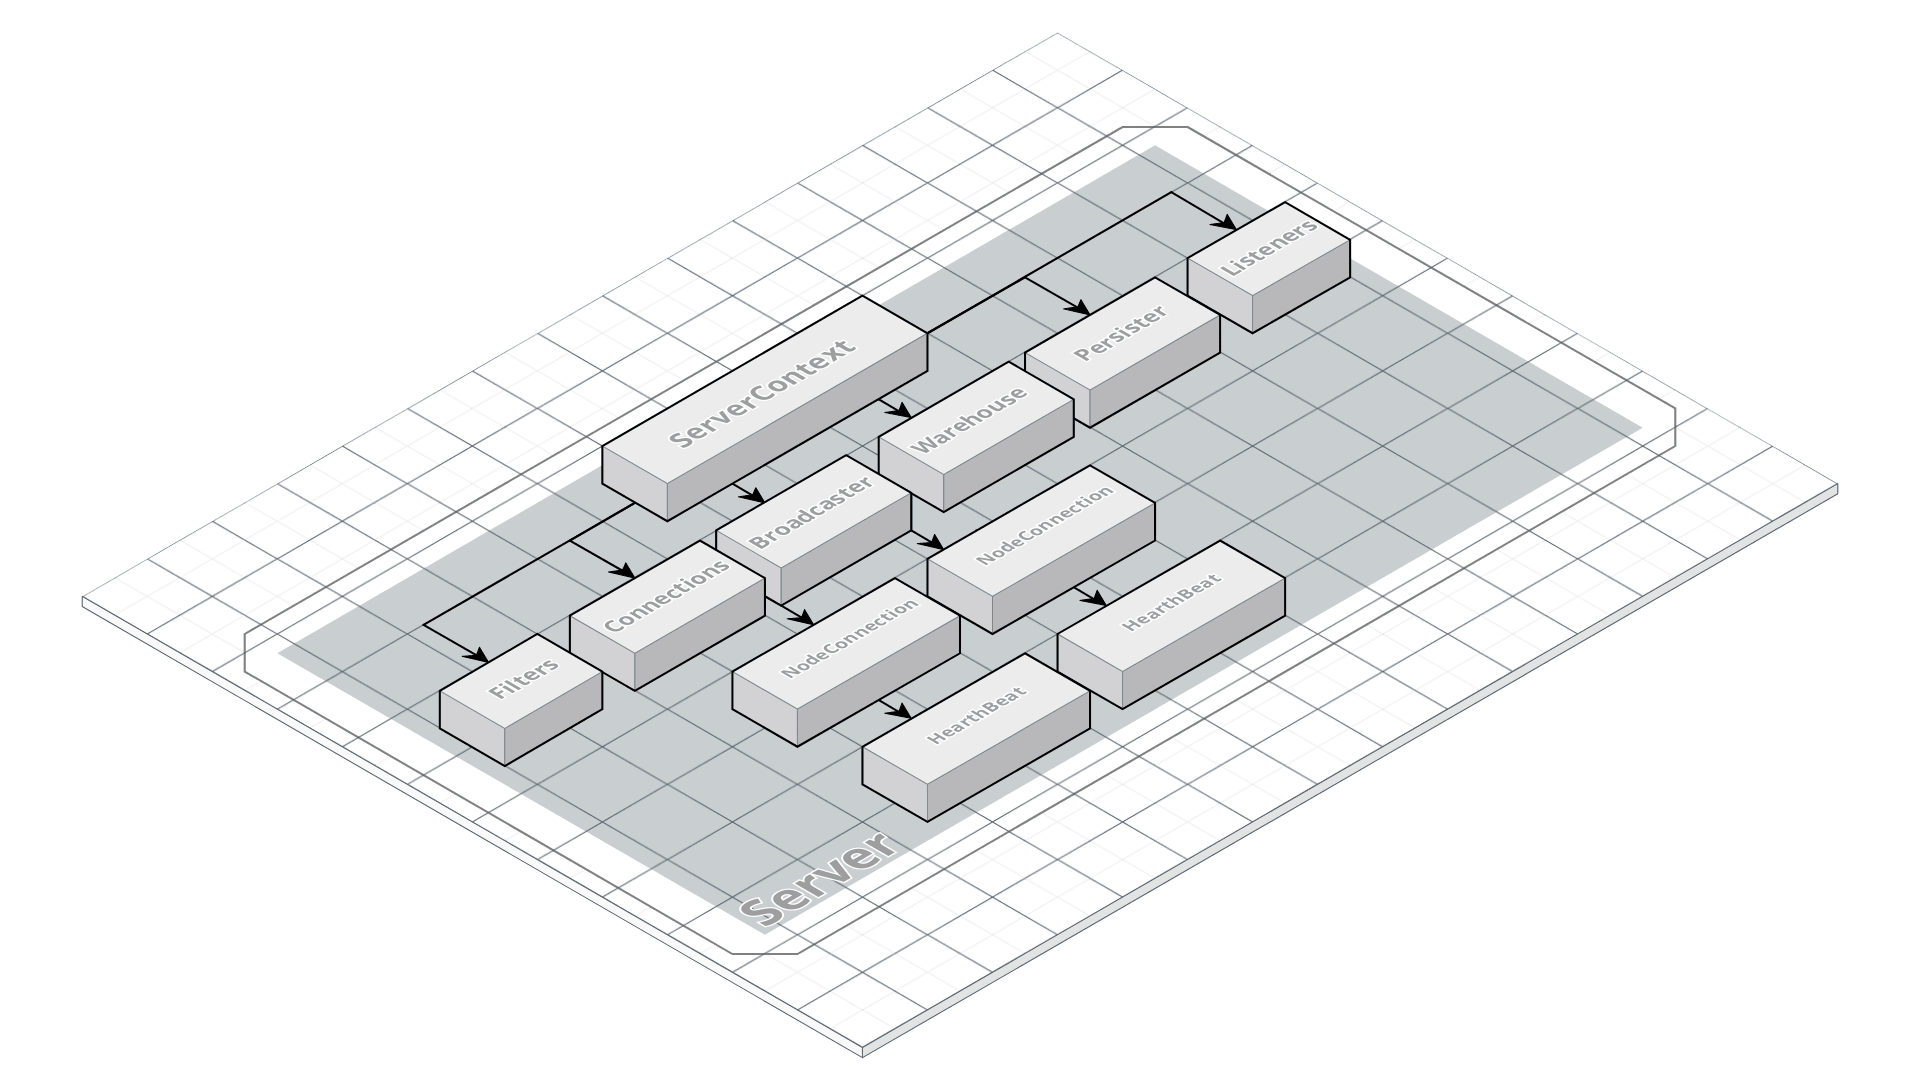
\includegraphics[width=\textwidth]{VS-Server-Context.png}
    
    \caption{Server-Context Aufbau}
    \label{}
\end{figure}

Sobald der ServerContext instanziiert wird, wird das Warehouse geladen. 
Zunächst wird versucht die Safe-Datei zu laden, scheitert das Laden wird das Warehouse leer instanziiert.
\lstinputlisting[linerange={53-64}, firstnumber=53]{../src/main/java/vs/chat/server/warehouse/Warehouse.java}

Das Warehouse hält sämtliche Daten, die persistiert werden müssen (z.\,B. Messages, Chats, Users). Der ServerContext erstellt außerdem den Persister. Der Persister ist ein Thread, der in regelmäßigen Abständen das Warehouse speichert.
\lstinputlisting[linerange={17-31}, firstnumber=17]{../src/main/java/vs/chat/server/persistence/Persister.java}
\lstinputlisting[linerange={66-75}, firstnumber=66]{../src/main/java/vs/chat/server/warehouse/Warehouse.java}
Alle Entitäten und Packete haben eine UUID (Universally Unique Identifier) um diese zu unterscheiden. Verweiße auf andere Entitäten (z.\,B. ein Chat hat mehrere Nutzer) werden Ähnlich zu Fremdschlüsseln in relationalen Datenbanken umgesetzt. Die Entität speichert nur die UUID der Verknüpfung und nicht direkt die Information. Dies erlaubt eine granularere Syncronisation und reduziert mögliche Konfliktsituationen zwischen verschiedenen Nodes. Eingesetzt werden UUIDv4, die pseudozufällig erstellt werden. Dadurch sind zwar theoretisch Konflikte möglich, jedoch in praxis sehr unwahrscheinlich.

Außerdem wird der Broadcaster erstellt, der die Verbindungen zu anderen Nodes hält und empfangene Nachrichten an diese verteilt.

\lstinputlisting[linerange={14-27}, firstnumber=14]{../src/main/java/vs/chat/server/node/NodeBroadcaster.java}


Weitere Variablen sind isCloseRequested, die die "endlos" Schleifen aller Threads steuert und connections, welche alle Connections zu Clients, die direkt zu dieser Node verbunden sind, hällt.

Der Nodebroadcaster erstellt bei Instanziierung je node einen eigenen Thread, der sich um das senden und das neu verbinden kümmert.
Nachrichten, die an eine Node gesendet werden soll werden sollen werden vom Broadcaster in die Queue geschrieben und die NodeConnection wird durch eine Semaphore aufgeweckt. 
Die NodeConnection versucht eine Nachricht zu senden. Scheitert das senden wird von einer Verbindungstrennung ausgegangen und die Verbindung wird neu verbunden.
\lstinputlisting[linerange={37-50}, firstnumber=37]{../src/main/java/vs/chat/server/node/NodeConnection.java}
Zusätzlich besitzt die NodeConnection jeweils einen HeartBeat-Thread.Dieser Thread sendet regelmäßig einen Ping um zu testen, ob die Verbindung noch steht.
\lstinputlisting[linerange={16-25}, firstnumber=16]{../src/main/java/vs/chat/server/node/NodeHeartBeatThread.java}

Nachdem nun alle initialisierungs Vorgänge abgeschlossen sind, kann der ServerSocket erstellt werden und clients akzeptiert werden.
Der Hauptserver-Thread ist dabei nur zuständig neue Verbindungen entgegenzunehmen. Für jede Verbindung wird ein ConnectionHandler-Thread erstellt, der sämtliche Nachrichten des Clients verarbeitet.
\lstinputlisting[linerange={41-60}, firstnumber=41]{../src/main/java/vs/chat/server/Server.java}

Nachrichten zwischen Servern und Clients werden als Packete ausgetauscht. Der Handler versucht dabei ein Packet vom Client zu lesen. Die Filter prüfen nun, ob das Packet gehandelt werden darf (und nach dem handeln werden diese aktualisiert).
\lstinputlisting[linerange={47-53}, firstnumber=47]{../src/main/java/vs/chat/server/ConnectionHandler.java}
Anschließend werden die passenden Listener gesucht und diese mit dem Packet aufgerufen.
\lstinputlisting[linerange={61-86}, firstnumber=61]{../src/main/java/vs/chat/server/ConnectionHandler.java}



Filter:
\begin{itemize}
    \item PacketIdFilter\\
        Der PacketId-Filter testet, ob ein Packet mit der Id bereits gesehen wurde. Nur wenn die Id neu ist darf das Packet gehandelt werden um rekursive Broadcasts zu vermeiden. Bereits gesehene Pakete werden im Warehouse mit gespeichert. Im seltenen Fall, dass die Node genau zwischen den Listenern und dem aktualisieren der Filter abstürzt kann es vorkommen, dass die gespeicherten Packet-ids nicht konsistenz zum Nutzdatenbestand sind. Hier könnte ein Transaktionsprotokoll implementiert werden. Da aber die Wahrscheinlichkeit dieses Fehlers äußerst gering ist wird hier darauf verzichtet.
        \lstinputlisting[linerange={9-17}, firstnumber=9]{../src/main/java/vs/chat/server/filter/PacketIdFilter.java}
\end{itemize}



Listener:
\begin{itemize}
    \item BaseEntityBroadcastListener\\
        Der Listener behandelt BaseEntityBroadcastPackete, die ausgestrahlt werden, sobald ein neuer Nutzer, ein neuer Chat oder eine neue Nachricht erstellt wird. Die empfangene Entität wird in das Warehouse aufgenommen und weiter gesendet, falls es dieser Node neu war.
        \lstinputlisting[linerange={22-28}, firstnumber=22]{../src/main/java/vs/chat/server/listener/BaseEntityBroadcastListener.java}
        Nachdem ein Chat erstellt wurde müssen die Clients, die an diesem Chat teilnehmen informiert werden. Da jede Node nur die direkt zu ihr verbundenen Clients kennt, muss jede Node prüfen ob sie einen teilnehmenden Client kennt und diesen informieren. Ähnliches gilt für neue Nutzer.
        \lstinputlisting[linerange={33-50}, firstnumber=33]{../src/main/java/vs/chat/server/listener/BaseEntityBroadcastListener.java}
    \item CreateChatListener\\
        Dieser Listener erstellt Chats anhand von einem CreateChatPacket. Sofern das Packet von einem Nutzer kommt wird ein neuer Chat mit allen Teilnehmern und dem Absender erstellt und weiter verteilt.
        \lstinputlisting[linerange={23-41}, firstnumber=23]{../src/main/java/vs/chat/server/listener/CreateChatListener.java}
    \item GetMessagesListener\\
        Mithilfe eines GetMessagePackets können alle Nachrichten abgefragt werden, die in einem Chat gesendet wurden.
        \lstinputlisting[linerange={20-32}, firstnumber=20]{../src/main/java/vs/chat/server/listener/GetMessagesListener.java}
    \item KeyExchangeListener\\
        Dieser Listener leitet KeyExchangePackete von einem Client an andere Clients weiter (gegebenenfalls über andere Nodes).
        \lstinputlisting[linerange={15-27}, firstnumber=15]{../src/main/java/vs/chat/server/listener/KeyExchangeListener.java}
    \item LoginListener\\
        Der LoginListener kümmert sich um die Authentifizierung eines Clients. Er prüft ob ein Nutzer besteht und falls ja wird das Passwort geprüft.
        Außerdem wird die Information der Connection gesetzt, zu welchem Client sie verbunden ist um ein gezieltes Senden zu ermöglichen (wie z.B. beim KeyExchange oder bei Messages).
        \lstinputlisting[linerange={25-34}, firstnumber=25]{../src/main/java/vs/chat/server/listener/LoginListener.java}
        Existiert noch kein Nutzer wird ein passender Nutzer erstellt.
        \lstinputlisting[linerange={37-56}, firstnumber=37]{../src/main/java/vs/chat/server/listener/LoginListener.java}
        Anschließend wird der Client auf den neuesten Stand gebracht indem ein LoginSyncPacket an den Client gesendet wird. Dieses enthält die User id des aktuellen Nutzers, die anderen registrierten Nutzer und alle Chats, an dem der Client teilnimmt.
        \lstinputlisting[linerange={59-65}, firstnumber=59]{../src/main/java/vs/chat/server/listener/LoginListener.java}
    \item MessageListener\\
        Messages, die vom Client an einen Chat gesendet werden werden von diesem Listener bearbeitet. Der Listener kümmert sich dabei auch um die Verteilung der Nachrichten an alle anderen Chatteilnehmer.
        \lstinputlisting[linerange={24-44}, firstnumber=24]{../src/main/java/vs/chat/server/listener/MessageListener.java}
    \item NodeSyncListener\\
        Wie in Fehlerbehandlung beschrieben müssen Nodes auf dem neuesten Stand gezogen werden, falls diese ausgefallen waren. Bei einem Reconnect wird ein NodeSyncPacket mit den aktuellen Informationen an die neu startende Node gesendet. Dieser Listener verarbeitet diese Packete indem er prüft ob eine Änderung vorliegt und wenn ja diese übernimmt und broadcastet. 
        \lstinputlisting[linerange={16-34}, firstnumber=16]{../src/main/java/vs/chat/server/listener/NodeSyncListener.java}
        Theoretisch kann es sein, dass ein Nutzer sich anmeldet bevor die Node ihre Synchronisation abgeschlossen hat. Dieser Fehlerfall wird aber nicht weiter behandelt, da die Synchronisationszeit und die Ausfallwahrscheinlichkeit einer Node als zu gering eingestuft wird.
\end{itemize}


Sollen hier andere Packete auch erkärt werden? Also Logout, GetMessageResponsePacket, NoOp, ...?

\subsection{Client}
//TODO


